\documentclass[]{article}
\usepackage{lmodern}
\usepackage{amssymb,amsmath}
\usepackage{ifxetex,ifluatex}
\usepackage{fixltx2e} % provides \textsubscript
\ifnum 0\ifxetex 1\fi\ifluatex 1\fi=0 % if pdftex
  \usepackage[T1]{fontenc}
  \usepackage[utf8]{inputenc}
\else % if luatex or xelatex
  \ifxetex
    \usepackage{mathspec}
  \else
    \usepackage{fontspec}
  \fi
  \defaultfontfeatures{Ligatures=TeX,Scale=MatchLowercase}
  \newcommand{\euro}{€}
\fi
% use upquote if available, for straight quotes in verbatim environments
\IfFileExists{upquote.sty}{\usepackage{upquote}}{}
% use microtype if available
\IfFileExists{microtype.sty}{%
\usepackage{microtype}
\UseMicrotypeSet[protrusion]{basicmath} % disable protrusion for tt fonts
}{}
\usepackage[margin=1in]{geometry}
\usepackage{hyperref}
\PassOptionsToPackage{usenames,dvipsnames}{color} % color is loaded by hyperref
\hypersetup{unicode=true,
            colorlinks=true,
            linkcolor=Maroon,
            citecolor=Blue,
            urlcolor=blue,
            breaklinks=true}
\urlstyle{same}  % don't use monospace font for urls
\usepackage{graphicx,grffile}
\makeatletter
\def\maxwidth{\ifdim\Gin@nat@width>\linewidth\linewidth\else\Gin@nat@width\fi}
\def\maxheight{\ifdim\Gin@nat@height>\textheight\textheight\else\Gin@nat@height\fi}
\makeatother
% Scale images if necessary, so that they will not overflow the page
% margins by default, and it is still possible to overwrite the defaults
% using explicit options in \includegraphics[width, height, ...]{}
\setkeys{Gin}{width=\maxwidth,height=\maxheight,keepaspectratio}
\setlength{\parindent}{0pt}
\setlength{\parskip}{6pt plus 2pt minus 1pt}
\setlength{\emergencystretch}{3em}  % prevent overfull lines
\providecommand{\tightlist}{%
  \setlength{\itemsep}{0pt}\setlength{\parskip}{0pt}}
\setcounter{secnumdepth}{0}

%%% Use protect on footnotes to avoid problems with footnotes in titles
\let\rmarkdownfootnote\footnote%
\def\footnote{\protect\rmarkdownfootnote}

%%% Change title format to be more compact
\usepackage{titling}

% Create subtitle command for use in maketitle
\newcommand{\subtitle}[1]{
  \posttitle{
    \begin{center}\large#1\end{center}
    }
}

\setlength{\droptitle}{-2em}
  \title{}
  \pretitle{\vspace{\droptitle}}
  \posttitle{}
  \author{}
  \preauthor{}\postauthor{}
  \date{}
  \predate{}\postdate{}


% Redefines (sub)paragraphs to behave more like sections
\ifx\paragraph\undefined\else
\let\oldparagraph\paragraph
\renewcommand{\paragraph}[1]{\oldparagraph{#1}\mbox{}}
\fi
\ifx\subparagraph\undefined\else
\let\oldsubparagraph\subparagraph
\renewcommand{\subparagraph}[1]{\oldsubparagraph{#1}\mbox{}}
\fi


\begin{document}

\section{Dr Nicholas J Clark}\label{dr-nicholas-j-clark}

Postdoctoral Fellow - University of Queensland, School of Veterinary
Science\\
Gatton, Queensland, Australia -
\href{mailto:nicholas.j.clark1214@gmail.com}{\nolinkurl{nicholas.j.clark1214@gmail.com}}
- 0432420979\\
\href{http://nicholasjclark.weebly.com/}{Homepage} -
\href{https://github.com/nicholasjclark}{GitHub} -
\href{https://scholar.google.com.au/citations?hl=en\&user=5bO9uxEAAAAJ\&view_op=list_works\&gmla=AJsN-F7bdYY9zcTVOHPEOVWZOJmCtgWpcxs_93x6Nxu1saXGdZjQLZ9byuM7Bdln9uk-HvNvAG1pThmdF6m_XgubeW0Q2sVTsjvpgou00G94hSHvb99iNTk}{Google
Scholar} -
\href{https://www.researchgate.net/profile/Nicholas_Clark4}{ResearchGate}

\subsection{Career Summary}\label{career-summary}

Flexible and engaging ecologist within interests in studying how
pathogen communities assemble, persist and function. Interested in
developing computational phylogenetic tools and adapting techniques from
statistical network theory to study how parasites interact with their
hosts across urban-wildlife gradients.

\subsection{Transferable Skills}\label{transferable-skills}

\begin{itemize}
\tightlist
\item
  Strong communication skills: 19 publications in peer-reviewed
  journals; four presentations at international conferences
\item
  Broad field experience: supervised teams of field researchers in both
  terrestrial and marine habitats
\item
  Extensive experience using script-based programming: proficient with
  frequentist and probabilistic statistical analyses; maintain two
  \texttt{R} packages for community ecology and landscape genetics
  research
\item
  Aptitude for leadership: trained four postgraduate students in
  bioinformatics and statistical techniques
\item
  Proven ability to obtain funding: \$52000 external funding from
  domestic and international organisations
\end{itemize}

\subsection{Qualifications}\label{qualifications}

\textbf{PhD}\\
\textbf{Griffith University} (Supervisors: Dr Sonya Clegg, Dr Robert
Adlard, Prof.~Hamish McCallum)\\
Thesis: \emph{The distribution and diversity of avian malaria parasites
in Australian and Southern Melanesian birds}

\begin{itemize}
\tightlist
\item
  Led field expeditions in diverse habitats on four islands in New
  Caledonia and across two Australian states
\item
  Acquired extensive experience coding biogeographical analyses on large
  datasets using frequentist and Bayesian techniques
\item
  Published ten peer-reviewed papers over four years, including six
  published chapters by submission of the thesis
\end{itemize}

\textbf{GDipResMeth}\\
\textbf{James Cook University} (Supervisors: Prof Garry Russ, Dr Lynne
van Herwerden) Thesis: \emph{Connectivity of butterflyfishes: pairing
molecular methods and field observations}

\begin{itemize}
\tightlist
\item
  Lead volunteer divers on two field trips to conduct marine abundance
  and habitat complexity surveys
\item
  Developed laboratory skills to conduct high-throughput genetic
  analyses
\item
  Obtained a high distinction in a Sampling and Experimental Design
  course and developed key programming skills to perform ecological
  statistical analyses
\end{itemize}

\textbf{BSc (honours)}\\
\textbf{University of North Carolina at Wilmington}; North Carolina, USA

\begin{itemize}
\tightlist
\item
  Dean's list for academic achievement in all semesters (GPA 4.0/4.0)
\end{itemize}

\pagebreak

\subsection{Professional Experience}\label{professional-experience}

\textbf{Postdoctoral Fellow (7/2016 - 12/18)}\\
\textbf{University of Queensland}, School of Veterinary Science

\begin{itemize}
\tightlist
\item
  Co-supervising two PhD students in disease ecology and quantitative
  genetics
\item
  Conducting research into the spatio-temporal evolution of canine
  parvoviruses
\item
  Leading a National Geographic-funded project on the spread of
  parasites at the human-wildlife interface
\end{itemize}

\textbf{Research Assistant (1/2016 - 7/16)}\\
\textbf{University of Queensland}, School of Veterinary Science
(Adviser: Dr Steven Kopp)

\begin{itemize}
\tightlist
\item
  Conducted molecular research into population genetics of canine
  hookworm
\item
  Established protocols to develop next generation sequencing tools for
  cat fleas
\end{itemize}

\textbf{Technical Laboratory Officer (fill-in for maternity leave;
9/2015 - 11/15)}\\
\textbf{Biosecurity Laboratory}, Queensland Dept. Agriculture and
Fisheries (Adviser: Dr Les Barker)

\begin{itemize}
\tightlist
\item
  Improved workflow efficiency by preparing reagents for three
  diagnostic laboratories
\item
  Cultured in-house microbe strains and carried out quality control
  testing
\end{itemize}

\subsection{Summary Citation Metrics}\label{summary-citation-metrics}

\begin{center}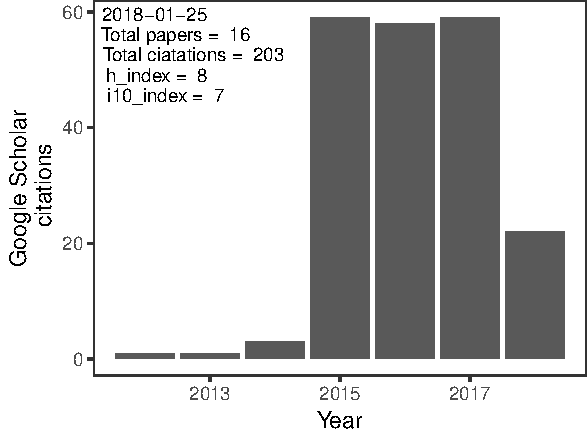
\includegraphics{NicholasClarkCV_files/figure-latex/unnamed-chunk-1-1} \end{center}

\pagebreak

\subsection{Full Publication List}\label{full-publication-list}

\textbf{2018}

\textbf{Clark, NJ}, Wells, K, and Lindberg, O. Unravelling changing
interspecific interactions across environmental gradients using Markov
random fields. \emph{Ecology} (accepted 02/03/18)

\textbf{Clark, NJ}. Phylogenetic uniqueness, not latitude, explains the
diversity of avian blood parasite communities worldwide. \emph{Global
Ecology and Biogeography} (accepted 27/02/18)

Wells, L, Gibson, DI, \textbf{Clark, NJ}, Ribas, A, Morand, S, McCallum,
H. Global spread of helminth parasites at the human -- domestic animal
-- wildlife interface. (2018). \emph{Global Change Biology} DOI:
10.1111/gcb.14064.
\href{http://nicholasjclark.weebly.com/uploads/4/4/9/4/44946407/wells_etal_2018_globchangbiol.pdf}{PDF}

\textbf{Clark, NJ}, Seddon, JM, Kyaw‐Tanner, M, Al-Alawneh, J, Harper,
G, McDonagh, P, and Meers, J. Emergence of canine parvovirus subtype 2b
(CPV-2b) infections in Australian dogs. \emph{Infection, Genetics and
Evolution} DOI: 10.1016/j.meegid.2017.12.013.
\href{http://nicholasjclark.weebly.com/uploads/4/4/9/4/44946407/clark_infgenevol_2018.pdf}{PDF}

\textbf{Clark, NJ}, Seddon, JM, Šlapeta, J, and Wells, K. Parasite
spread at the domestic animal - wildlife interface: anthropogenic
habitat use, phylogeny and body mass drive risk of cat and dog flea
(Ctenocephalides spp.) infestation in wild mammals. \emph{Parasites \&
Vectors} DOI: 10.1186/s13071-017-2564-z.
\href{http://nicholasjclark.weebly.com/uploads/4/4/9/4/44946407/clark_etal_2018parvec.pdf}{PDF}

\textbf{2017}

\textbf{Clark, NJ}, Clegg, SM, Sam, K, Goulding, W, Koane, B and Wells,
K. Climate, host phylogeny and the connectivity of host communities
govern regional parasite assembly. \emph{Diversity and Distributions}
DOI: 10.1111/ddi.12661.
\href{http://nicholasjclark.weebly.com/uploads/4/4/9/4/44946407/clark_et_al-2017-diversity_and_distributions.pdf}{PDF}

\textbf{Clark, NJ} and Clegg, SM (2017) Integrating phylogenetic and
ecological distances reveals new insights into parasite host
specificity. \emph{Molecular Ecology} 26(11), 3074-3086.
\href{http://nicholasjclark.weebly.com/uploads/4/4/9/4/44946407/clark_and_clegg-2017-molecular_ecology.pdf}{PDF}

McKee, J, \textbf{Clark, NJ}, Shapter, F and Simmons, G. (2017) A new
look at the origins of Gibbon Ape Leukemia Virus. \emph{Virus Genes}
53(2), 165-172.
\href{http://nicholasjclark.weebly.com/uploads/4/4/9/4/44946407/mckee_et_al._2017_virus_genes.pdf}{PDF}

\textbf{2016}

\textbf{Clark, NJ}, Wells, K, Dimitrov, D and Clegg, SM. (2016)
Co-infections and environmental conditions drive the distributions of
blood parasites in wild birds. \emph{Journal of Animal Ecology} 85(6),
1461-1470.
\href{http://nicholasjclark.weebly.com/uploads/4/4/9/4/44946407/clark_et_al-2016-journal_of_animal_ecology.pdf}{PDF}

Aharon-Rotman, Y, Buchanan, KL, \textbf{Clark, NJ}, Klaassen, M and
Buttemer, WA. (2016) Why fly the extra mile? Using stress biomarkers to
assess wintering habitat quality in migratory shorebirds.
\emph{Oecologia} 182(2), 385-395.
\href{http://nicholasjclark.weebly.com/uploads/4/4/9/4/44946407/aharon-rotmanetal.2016whyflyextramile.pdf}{PDF}

Goulding, W, Adlard, RD, Clegg, SM and \textbf{Clark, NJ}. (2016)
Molecular and morphological description of \emph{Haemoproteus}
(\emph{Parahaemoproteus}) \emph{bukaka} (species nova), a haemosporidian
associated with the strictly Australo-Papuan host Subfamily Cracticinae.
\emph{Parasitology Research} 115,
3387-3400.\href{http://nicholasjclark.weebly.com/uploads/4/4/9/4/44946407/goulding_et_al_parasres2016.pdf}{PDF}

\textbf{Clark, NJ}, Clegg, SM and Klaassen, M. (2016) Migration strategy
and pathogen risk: non‐breeding distribution drives malaria prevalence
in migratory waders. \emph{Oikos} 125(9), 1358-1368.
\href{http://nicholasjclark.weebly.com/uploads/4/4/9/4/44946407/clark_et_al-oikos_2016.pdf}{PDF}

\textbf{2015}

\textbf{Clark, NJ}, Ishtiaq, F, Olsson-Pons, S and Clegg, SM. (2015)
Specialist enemies, generalist weapons and the potential spread of
exotic pathogens: malaria parasites in a highly invasive bird.
\emph{International Journal for Parasitology} 45(14), 891-899.
\href{http://nicholasjclark.weebly.com/uploads/4/4/9/4/44946407/clark_et_al_ijp_2015_mynas.pdf}{PDF}

Olsson-Pons, S, \textbf{Clark, NJ}, Ishtiaq, F and Clegg, SM. (2015)
Differences in host species relationships and biogeographical influences
produce contrasting patterns of prevalence, community composition and
genetic structure in two genera of avian malaria parasites in southern
Melanesia. \emph{Journal of Animal Ecology} 84(4), 985-998.
\href{https://nicholasjclark.weebly.com/uploads/4/4/9/4/44946407/olsson-pons_et_al-2015-journal_of_animal_ecology.pdf}{PDF}

\textbf{Clark, NJ}, Adlard, RD and Clegg, SM. (2015) Molecular and
morphological characterization of \emph{Haemoproteus}
(\emph{Parahaemoproteus}) \emph{ptilotis}, a parasite infecting
Australian honeyeaters (Meliphagidae), with remarks on prevalence and
potential cryptic speciation. \emph{Parasitology Research} 114(5),
1921-1928.
\href{http://nicholasjclark.weebly.com/uploads/4/4/9/4/44946407/clark_et_al_paras_res_2015.pdf}{PDF}

\textbf{Clark, NJ} and Clegg, SM. (2015) The influence of vagrant hosts
and weather patterns on the colonisation and persistence of blood
parasites in an island bird. \emph{Journal of Biogeography} 42(4),
641-651.
\href{http://nicholasjclark.weebly.com/uploads/4/4/9/4/44946407/clark_and_cleggjbi_proofs.pdf}{PDF}

\textbf{2014}

\textbf{Clark, NJ}, Adlard, RD and Clegg, SM. (2014) First evidence of
avian malaria in Capricorn Silvereyes (\emph{Zosterops lateralis
chlorocephalus}) on Heron Island. \emph{The Sunbird} 44, 1-11
\href{http://nicholasjclark.weebly.com/uploads/4/4/9/4/44946407/sunbird_44_1__avian_malaria_author_copy.pdf}{PDF}

\textbf{Clark, NJ}, Clegg, SM and Lima, MR. (2014) A review of global
diversity in avian haemosporidians (Plasmodium and Haemoproteus:
Haemosporida): new insights from molecular data. \emph{International
Journal for Parasitology} 44(5), 329-338
\href{http://nicholasjclark.weebly.com/uploads/4/4/9/4/44946407/clark_et_al_ijp_2014_published_version.pdf}{PDF}

\textbf{2012}

\textbf{Clark, NJ} and Russ, GR. (2012) Ontogenetic shifts in the
habitat associations of butterflyfishes (F. Chaetodontidae).
\emph{Environmental Biology of Fishes} 94, 579-590

\subsection{Publications in Review}\label{publications-in-review}

\textbf{Clark, NJ} and Soares Magalhães, RJ. Airborne geographical
dispersal of Q Fever from livestock holdings to human communities: a
systematic review and critical appraisal of evidence. \emph{BMC
Infectious Diseases} (1st submission 18/02/18)

Wells, K, Gibson, D, and \textbf{Clark, NJ}. Global patterns in helminth
host specificity: phylogenetic and functional diversity of regional host
species pools matter. \emph{Ecography} (1st submission 25/01/18)

Lawrence, AL, Webb, CE, \textbf{Clark, NJ}, Halajian, A, Mihalca, A,
Miret, J, D'Amico, G, Brown, G, Kumsa, B, Modry, D, and Šlapeta, J.
Out-of-Africa origins and global climatic distribution of the common cat
flea, Ctenocephalides felis: the hitchhiker's guide to world domination.
\emph{Molecular Phylogenetics and Evolution} (1st submission 26/11/17)

\subsection{Service and Discipline
Involvement}\label{service-and-discipline-involvement}

\textbf{Service}

\begin{itemize}
\tightlist
\item
  Served as panel member to mark a UQ Honour's thesis
\item
  Contributed to teaching and assignment design for three undergraduate
  courses at the School of Veterinary Science
\item
  Currently co-supervising two PhD students
\item
  Acted as student volunteer for the 2017 Australian Society for
  Parasitology International Conference
\end{itemize}

\textbf{Referee}

\begin{itemize}
\tightlist
\item
  \emph{Ecology Letters}
\item
  \emph{Molecular Biology and Evolution}
\item
  \emph{Evolutionary Ecology}
\item
  \emph{Journal of Biogeography}
\item
  \emph{International Journal for Parasitology}
\item
  \emph{Journal of Parasitology}
\item
  \emph{Journal of Animal Ecology}
\item
  \emph{Infection, Genetics and Evolution}
\item
  \emph{Parasitology}
\item
  \emph{Malaria Journal}
\item
  \emph{Parasites \& Vectors}
\end{itemize}

\subsection{Funding Support}\label{funding-support}

\textbf{2017}

\textbf{\$US18,400}: National Geographic Scientific Research Grant
(co-authored the proposal). Tracing the spillover of fleas and paralysis
ticks between wildlife and domestic pets in Australia

\textbf{2015}

\textbf{\$AU4,975}: Birds Queensland Research Award (co-authored the
proposal). The role of invasive birds as carriers of exotic pathogens;
implications for co-occurring native birds

\textbf{\$AU3,125}: BirdLife Australia Stuart Leslie Bird Research Award
(authored the proposal). Enemy release or novel weapons: malaria's role
in the spread of the invasive Indian Myna

\textbf{2014}

\textbf{\$AU2,000}: Griffith University Environmental fund for impactful
publications

\textbf{2013}

\textbf{\$US20,250}: National Geographic Scientific Research Grant
(co-authored the proposal). Avian malaria in southern Melanesian birds

\textbf{2012}

\textbf{\$AU3,750}: BirdLife Australia Stuart Leslie Bird Research Award
(authored the proposal). Avian malaria lineage distribution, diversity
and host specificity in southeast Queensland

\textbf{\$AU5,000}: Birds Queensland Research Award (authored the
proposal). The prevalence, distribution and diversity of avian malaria
parasites in southeast Queensland

\textbf{\$AU78,000}: Griffith University International Postgraduate
Research Award

\subsection{Teaching Contributions}\label{teaching-contributions}

\textbf{2017}

\textbf{University of Queensland}, Gatton Campus: Ecological and Disease
Genetics (Course Coordinator)\\
Undergraduate (3rd year Science), semester 1

\begin{itemize}
\tightlist
\item
  Planned learning objectives; wrote the electronic course profile (ECP)
  and all assignments
\item
  Delivered flexible, interactive lectures and tutorials that were
  well-received by students
\item
  Achieved overwhelmingly positive feedback on student evaluations,
  including scores of `Outstanding' for teacher ratings
\item
  SECaTs available at: VETS3042/Ecological and Disease
  Genetics/6720/23028
\end{itemize}

\textbf{University of Queensland}, Gatton Campus: Animal Breeding and
Genetics (Course Coordinator)\\
Undergraduate (Bachelor of Veterinary Medicine), semester 2

\begin{itemize}
\tightlist
\item
  Planned learning objectives; contributed to preparation of assignments
  and end of semester exam
\item
  Independently lead theory-based genetics tutorials
\item
  Nominated for a `Golden Speculum' Best Lecturer award for 2017
\end{itemize}

\textbf{2016 - 17}

\textbf{University of Queensland}, Gatton Campus: Molecular and
Quantitative Plant Genetics; Molecular and Quantitative Animal Genetics
(Lead tutor)\\
Undergraduate (2nd year Science and 2nd year Agriculture), semester 2

\begin{itemize}
\tightlist
\item
  Independently lead laboratory and theory tutorials
\item
  Marked assignments and liaised with course coordinators to enhance
  curriculums
\end{itemize}

\textbf{2015 - 17}

\textbf{University of Queensland}, Gatton Campus: Animal Breeding and
Molecular Genetics; Animal Pathogens and Immunity; Principles of Disease
(Assistant tutor)\\
Undergraduate (2nd year Veterinary Science), semesters 1 and 2

\begin{itemize}
\tightlist
\item
  Collaborated with fellow tutors to lead laboratory and theory
  tutorials
\item
  Marked assignments
\end{itemize}

\textbf{2013}

\textbf{Griffith University}, Gold Coast Campus: Ecology; Earth Sciences
(Assistant tutor)\\
Undergraduate (2nd year Science), semester 2

\begin{itemize}
\tightlist
\item
  Independently lead laboratory and theory tutorials
\end{itemize}

\subsection{Mentoring And Research
Training}\label{mentoring-and-research-training}

\textbf{2017 - present}

Co-supervising UQ PhD student (A. McGowan), studying population genomics
of dugongs. This student is developing novel landscape genetics analyses
and recently qualified for Faculty-level heats in the UQ Three Minute
Thesis competition

\textbf{2016 - present}

Co-supervising UQ PhD student (T. Proboste), studying population
genomics and host-parasite interactions in paralysis ticks. This student
is adapting social science methods to study host-pathogen interactions,
and has already presented at two conferences

\textbf{2014 - 16}

Trained UQ PhD student (W. Goulding) in molecular techniques and aided
project design, resulting in two collaborative papers (both in
Parasitology Research) and one successful co-authored grant proposal
(Birds Queensland; \$AU4975)

\textbf{2014}

Trained Deakin University PhD student (Y. Aharon-Rotman) in Bayesian
phylogenetic modelling, resulting in one collaborative paper (Oecologia)

\textbf{2012 - 13}

Trained Griffith University honour's student (S. Olsson-Pons) in
bioinformatics, resulting in two collaborative papers (Journal of Animal
Ecology; International Journal for Parasitology)

\subsection{Presentations and Societal
Impacts}\label{presentations-and-societal-impacts}

\textbf{2017}

Oral presentation: Australian Society for Parasitology Conference,
Leura, Australia

\textbf{2016}

Research used to frame a Question Without Notice in NSW Parliament, from
Shooters and Fishers Party MP to the Minister for Primary Industries

Oral presentation: Griffith University Wildlife Disease Ecology Group,
Brisbane, Australia

\textbf{2015}

Interviewed on ABC Radio National and ABC Radio Gold Coast regarding
research on exotic malaria strains spread by invasive birds

Interviewed for feature stories in the Australian Society for
Parasitology quarterly newsletter and in Australian Birdlife regarding
research on avian malaria in Australian birds

Oral presentation: University of Queensland ARC Cavity Nesting Group,
Brisbane, Australia

Oral presentation: Evolutionary Ecology of Infectious Diseases
Conference, Athens, USA

Oral presentation: Griffith University Wildlife Disease Ecology Group,
Brisbane, Australia

Poster presentation: Wildlife Disease Association Conference, Sunshine
Coast, Australia

\textbf{2014}

Oral presentation: Queensland Ornithological Society, Brisbane,
Australia

Oral presentation: Australian Society for Parasitology Concepts in
Parasitology Workshop, Canberra, Australia.

Taught diagnostic techniques to students in a Parasitology High School
Outreach Program at Ulladulla High School, Ulladulla, NSW, Australia

\textbf{2013}

Oral presentation: Centre for Integrative Ecology, Deakin University,
Geelong, Australia

Poster presentation: Malaria and Related Haemosporidians of Wildlife
International Conference, Vilnius, Lithuania

\subsection{Honours and Awards}\label{honours-and-awards}

\textbf{2017}

Invited to act as co-chair for a Wildlife Parasitology session at the
Australian Society for Parasitology Conference, Leura, Australia

\textbf{2016}

Research article featured on the cover and on the Editor's Choice list
at International Journal for Parasitology

\textbf{2014}

1st place oral presentation; Griffith University School of Environment
Student Symposium

\textbf{2014}

Accepted for competitive placement with travel funds; Australian Society
for Parasitology Concepts in Parasitology Workshop, Canberra, Australia

\textbf{2012}

2nd place oral presentation; Griffith University School of Environment
Student Symposium

\textbf{2012}

Accepted for competitive placement with travel funds; Malaria RCN
Student Workshop, Virginia, USA

\subsection{Relative to Opportunity}\label{relative-to-opportunity}

I completed my undergraduate degree (Bachelor of Science; GPA 4.0) in
2009 and completed a Graduate Diploma by Research Methods in 2011 (High
Distinction average). I began my PhD in February 2012 and finished in
April 2016, delivering a thesis with six published chapters and two
published appendices. My PhD work provided new insights into mechanisms
driving the distributions of blood parasites in wild birds. I also
gained a broad understanding of coexistence theory and its applications
to community ecology, for instance by providing evidence that
interspecific parasite interactions can influence infection rates.

Following my PhD I have devoted much of my postdoctoral work to teaching
and mentoring postgraduate research students. This has provided me with
a set of leadership and organizational skills that I believe is unique
among my peers. It also taught me to be proficient with the time that I
do have available for research. Since winding down teaching in July last
year, I have published seven papers and submitted another three,
bringing my total to 19 publications. The quality and significance of
this work is reflected by my exemplary publication record in some of the
top journals in Ecology and Biogeography. My research has also garnered
international recognition. I was invited to present work on new
statistical tools for studying parasite niche differentiation at the
Australian Society for Parasitology's 2017 International Conference,
where I was also invited to act as co-chair for a wildlife parasitology
session. Recently, I have been invited to act as guest editor for a
\href{http://www.mdpi.com/journal/tropicalmed/special_issues/Medical_Geography}{\emph{Tropical
Medicine and Infectious Disease} Special Issue} on disease patterns in a
changing environment.

\subsection{Referees}\label{referees}

\begin{itemize}
\tightlist
\item
  A/Prof Jennifer Seddon, UQ Gatton Campus;
  \href{mailto:j.seddon1@uq.edu.au}{\nolinkurl{j.seddon1@uq.edu.au}}
\item
  Dr Robert Adlard, Queensland Museum;
  \href{mailto:robert.adlard@qm.qld.gov.au}{\nolinkurl{robert.adlard@qm.qld.gov.au}}
\item
  Dr Sonya Clegg, Oxford University;
  \href{mailto:sonya.clegg@zoo.ox.ac.uk}{\nolinkurl{sonya.clegg@zoo.ox.ac.uk}}
\item
  Prof Marcel Klaassen, Deakin University;
  \href{mailto:marcel.klaassen@deakin.edu.au}{\nolinkurl{marcel.klaassen@deakin.edu.au}}
\end{itemize}

\end{document}
